% ||||||||||||||||||||||||||||||||||||||||||||||
% Capitulo de Revisão Bibliográfica
% ||||||||||||||||||||||||||||||||||||||||||||||

\chapter{Revisão Bibliográfica}

Com o objetivo de compreender os conceitos básicos do trabalho, este capítulo os apresenta de forma evolutiva e 
cronológica, partindo dos conceitos sobre motores elétricos com suas particularidades, até o estado da arte em 
detecção e diagnóstico de falhas em motores elétricos de indução. 


%++++++++++++++++++++++++++++++++++++++++++++++++++++++++++++++++
% 
%++++++++++++++++++++++++++++++++++++++++++++++++++++++++++++++++

\section{Motores Elétricos de Indução}\label{sec:}

Motores elétricos de indução são um dos tipos de máquinas elétricas, as quais convertem energia elétrica em mecânica. 
Nos motores elétricos de indução, uma corrente elétrica é induzida no rotor através da corrente de armadura que circula
no estator. Contudo, um rotor do tipo gaiola de esquilo, pode ser visto na figura \ref{fig:ind_motor_petruzella_p115}, 
é um curto-circuito formado por barras e lâminas de alumínio. Por essa constituição simples, motores elétricos de indução
com rotor do tipo gaiola resultam em motores relativamente baratos e confiáveis, contribuindo para sua popularidade \cite{Umans2003}.
 
\begin{figure}[H]
    \caption{Motor elétrico de indução tipo gaiola de esquilo.}
    \begin{center}
        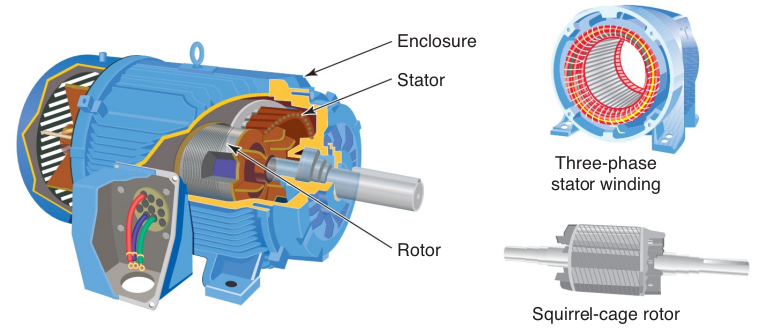
\includegraphics[scale=.5]{referencial/img/ind_motor_petruzella_p115.png}
    \end{center}
    \fonte{\citeonline{Petruzella1911}.} 
    \label{fig:ind_motor_petruzella_p115}
\end{figure}

Uma das formas de se modelar um motor elétrico de indução, é através de uma representação em forma de um circuito 
elétrico, onde todas as variáveis podem ser representadas por componentes elétricos simples, facilitando a compreensão, modelagem e
prever possíveis variações nos elementos mecânicos e elétricos. O circuito representado na figura \ref{fig:circuit_fitzgerald_p354},
é um circuito equivalente monofásico de um motor elétrico indutivo polifásico, o que simplifica toda a análise em um único circuito,
onde é trivial isolar a tensão em um terminal e a sua corrente. Para se saber as demais correntes e tensões, basta deslocar as fases
em $\pm\ang{120}$ \cite{Umans2003}.

\begin{figure}[H]
    \caption{Circuito equivalente monofásico de um motor de indução polifásico.}
    \begin{center}
        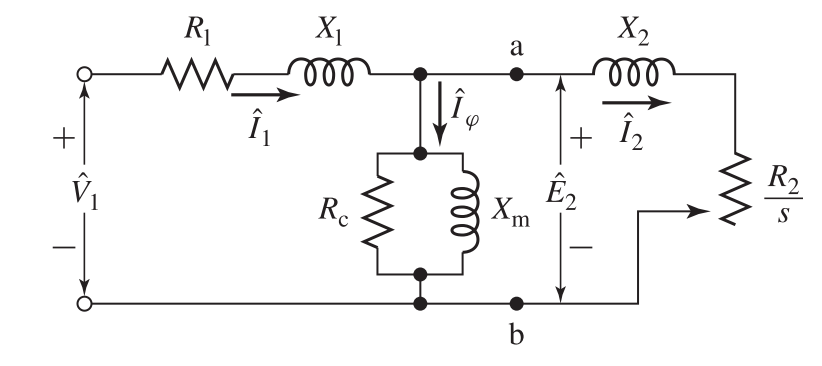
\includegraphics[scale=.35]{referencial/img/circuit_fitzgerald_p354.png}
    \end{center}
    \fonte{\citeonline{Umans2003}.} 
    \label{fig:circuit_fitzgerald_p354}
\end{figure}

Onde

\begin{itemize}
    \item $\hat{V}_1$ = tensão no estator
    \item $\hat{E}_2$ = Força eletromotriz contrária gerada pelo fluxo no entreferro
    \item $\hat{I}_1$ = corrente do estator
    \item $\hat{R}_1$ = resistência efetiva do estator
    \item $\hat{X}_1$ = reatância de vazamento do estator
    \item $R_c$ = resistência às perdas no núcleo
    \item $X_m$ = reatância magnetizante
    \item $\hat{I}_2$ = componente de corrente gerada pela carga
    \item $\hat{X}_2$ = reatância de vazamento do rotor no estator na frequência de escorregamento
    \item $R_2$ = resistência do rotor
    \item $\hat{I}_\varphi$ = componente de corrente excitada no estator
\end{itemize}

Com a apresentação de conceitos básicos sobre motores elétricos de indução e sua modelagem, é possível abordar os principais falhas que 
acometem as partes mecânicas e elétricas de um motor elétrico.


%----------------------------------------------------------------
% 
%----------------------------------------------------------------

\section{Falhas em Motores Elétricos de Indução}\label{sec:}

Como dito anteriormente, um motor elétrico é utilizado para transformar energia elétrica em mecânica, sendo empregado em máquinas que podem
realizar diversas atividades. A figura \ref{fig:monitoring_methods_rilski_p78} representa uma generalização de um sistema em que um motor
elétrico é empregado. Nesta figura, podemos ver os elementos que constituem a parte elétrica: a fonte de energia, o inversor de frequência e
o próprio motor. Também é possível ver a parte mecânica: a estrutura do motor, o acoplamento mecânico, a carga e as bases. Todos esses
elementos podem induzir falhas no motor, começando pelo acionamento, onde pode ocorrer uma falha e fazer o motor perder uma fase, ou ainda, 
oscilações na tensão e sobre carga. Todas essas falhas inevitavelmente alteram o espectro da fonte de energia \citeonline{Gorbounov2018}. 
Na parte mecânica, o desalinhamento entre a carga e o motor pode acarretar falhas no acoplamento que transfere a energia mecânica do motor
para o processo, e isso é normalmente provocado por uma instalação inapropriada.

\begin{figure}[H]
    \caption{Visão geral de sistema com um motor elétrico.}
    \begin{center}
        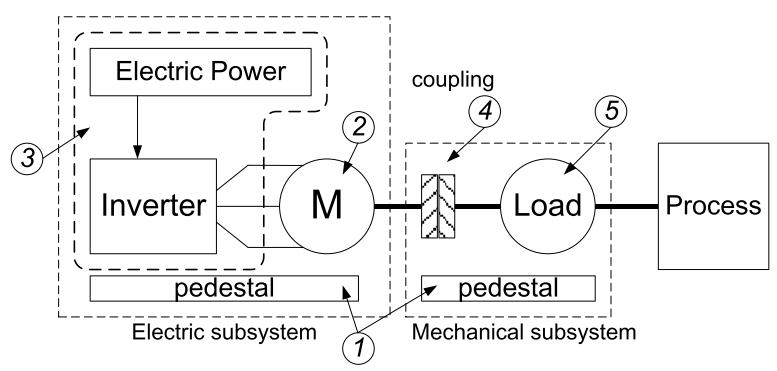
\includegraphics[scale=.45]{referencial/img/motor_system_rilski_p2.png}
    \end{center}
    \fonte{\citeonline{Gorbounov2018}.} 
    \label{fig:motor_system_rilski_p2}
\end{figure}

A figura \ref{fig:faults_rilski_p77} apresenta uma árvore das principais falhas que acometem os motores elétricos, sendo também divididas
em mecânicas e elétricas. 

\begin{figure}[H]
    \caption{Árvo dos principais tipos de falhas em motores elétricos.}
    \begin{center}
        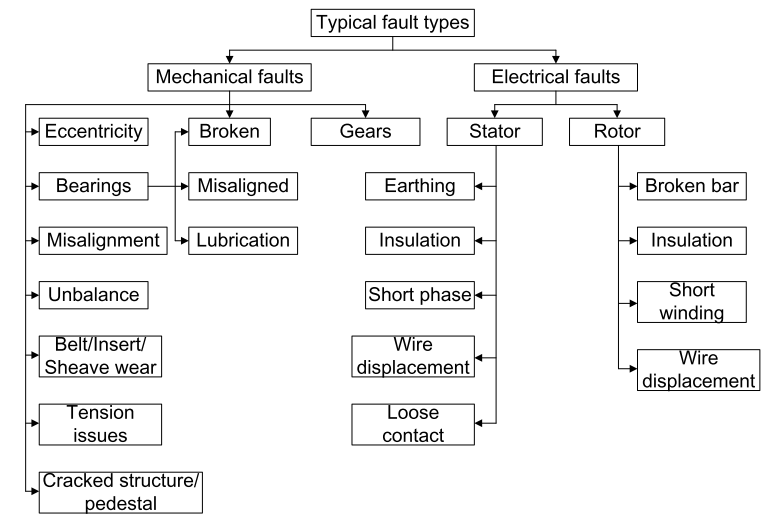
\includegraphics[scale=.45]{referencial/img/faults_rilski_p77.png}
    \end{center}
    \fonte{\citeonline{Gorbounov2018}.} 
    \label{fig:faults_rilski_p77}
\end{figure}

Dentre todas essas falhas, o trabalho aborda com maior foco as falhas mecânicas, mais especificamente desalinhamento, rolamentos 
e desbalanceamento que causam um aumento na vibração do sistema. O desalinhamento ocorre quando o motor e o sistema não estão perfeitamente alinhados, podendo ter dois tipos:
paralelo e angulas, os quais podem ser vistos na figura \ref{fig:misadraw_analog_p2}, respectivamente na parte a) e b) 
\cite{Sopcik2019}.

\begin{figure}[H]
    \caption{Ilustração com os tipos de desalinhamento.}
    \begin{center}
        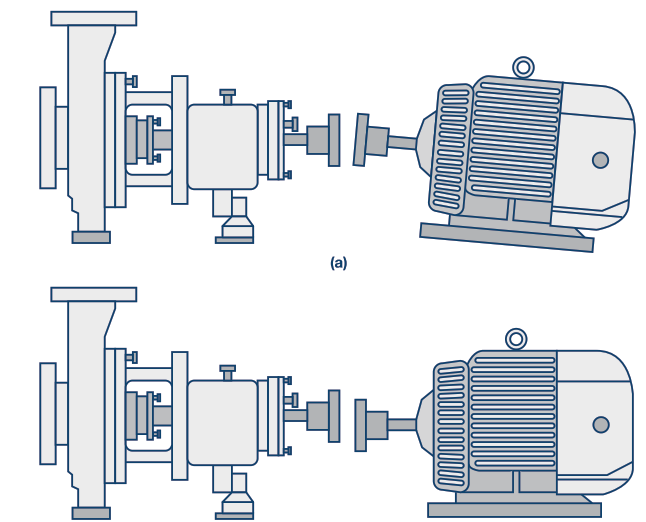
\includegraphics[scale=.35]{referencial/img/misadraw_analog_p2.png}
    \end{center}
    \fonte{\citeonline{Sopcik2019}.} 
    \label{fig:misadraw_analog_p2}
\end{figure}

Já a falha de desbalanceamento, pode ocorrer em qualquer parte rotativa do sistema, que vai desde o motor até a carga, compreendida por
algum problema na disposição das massas. Por último, os rolamentos, que são utilizados em diversas partes de um sistema e que podem
apresentar pequenas rachaduras na falta de lubrificação, que podem ser vistas na figura \ref{fig:bearing_analog_p3}, aumentando a 
vibração \cite{Sopcik2019}.

\begin{figure}[H]
    \caption{Imagens de rolamentos no topo, e falhas na parte de baixo.}
    \begin{center}
        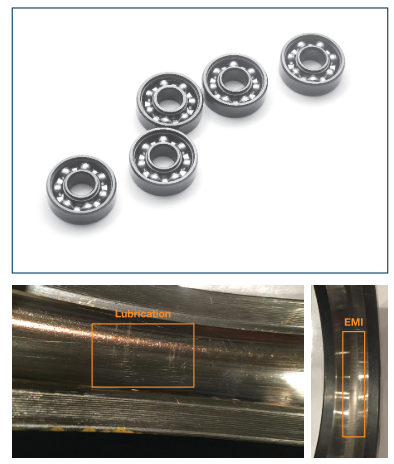
\includegraphics[scale=.5]{referencial/img/bearing_analog_p3.png}
    \end{center}
    \fonte{\citeonline{Sopcik2019}.} 
    \label{fig:bearing_analog_p3}
\end{figure}

Mais de 66\% destas falhas são detectadas durante a operação e 28\% são encontradas apenas durante a manutenção 
preventiva \cite{Gorbounov2018}, destacando a importância de uma boa estratégia de manutenção. Existem três tipos de estratégias 
para manutenção \cite{Wu2013}:  

\begin{enumerate}
    \item Funcionar até quebrar: é uma das técnicas mais tradicionais, onde o equipamento funciona até quebrar. Só após isso a
manutenção é realizada. Possui diversas desvantagens, principalmente pelo fato que a falha pode se manifestar durante a produção e
deixar a máquina parada por horas, causando grande prejuízo;
    \item Manutenção Preventiva: é baseada em manutenções em intervalos regulares antes da falha se manifestar. Quando a frequência das
falhas é conhecida, pode ser uma boa estratégia, mas possibilita a troca de componentes que ainda teriam uma sobrevida, ou ainda, a falha
ocorrer antes do previsto, devido à alterações não esperada no processo;
    \item Manutenção Preditiva: quando é detectado que uma falha está próxima, antes de acontecer e com tempo ótimo para se fazer a 
manutenção sem afetar a produtividade e danificar mais o equipamento. Essa estratégia é baseada em um monitoramento do equipamento,
permitindo acompanhar o estado de saúde da máquina. Se bem implementa essa estratégia, pode reduzir em até 65\% os custos de manutenção
\cite{Wu2013};
\end{enumerate}

Após apresentados os conceitos básicos sobre motores elétricos e suas falhas, e como essas falhas aumentam o nível de vibração,
o próximo capítulo tem por objetivo apresentar conceitos de detecção e diagnóstico destas falhas.


%++++++++++++++++++++++++++++++++++++++++++++++++++++++++++++++++
% 
%++++++++++++++++++++++++++++++++++++++++++++++++++++++++++++++++

\section{Sistemas de Detecção e Diagnóstico de Falhas}\label{sec:}

Como apresentado anteriormente, falhas em componentes de um motor elétrico, ou no sistema em que ele está inserido, podem ocasionar
um aumento da vibração e alteração no espectro da corrente do motor, que serão estudados na sequência.


%----------------------------------------------------------------
% 
%----------------------------------------------------------------

\subsection{Análise de Vibração}\label{subsec:}

O aumento da vibração pode ocasionar perturbações até mesmo na parte elétrica de um motor, como mostra o gráfico que está na 
figura \ref{fig:fault_effect_randall_p54}. Com o aumento da carga e da vibração em conjunto, o efeito mecânico e elétrico pode ser 
severo \citeonline{Wu2013}.

\begin{figure}[H]
    \caption{Variação da carga para distinção da causa do efeito observado.}
    \begin{center}
        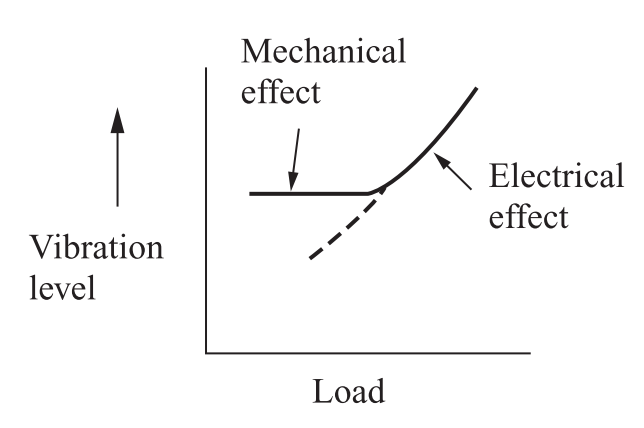
\includegraphics[scale=.45]{referencial/img/fault_effect_randall_p54.png}
    \end{center}
    \fonte{\citeonline{Wu2013}.} 
    \label{fig:fault_effect_randall_p54}
\end{figure}


Essa vibração possui um característica específica, que depende de qual falha ela é oriunda, que acaba criando uma assinatura
ao se analisar a vibração, sendo possível diagnosticar se o motor e o sistema em que ele está inserido está com boa saúde \cite{Wu2013}.
Uma das primeiras técnicas para classificar o estado de saúde de uma máquina, é a norma ISO 10816-1, que recomenda níveis de vibração 
em valores eficaz de acordo com o porte da máquina, que pode ser visto na figura \ref{fig:iso10816-1_randall_p146}.

\begin{figure}[H]
    \caption{Tabela de valores eficaz máximos de velocidade para cada porte de máquina indicados pela norma ISO 10816-1.}
    \begin{center}
        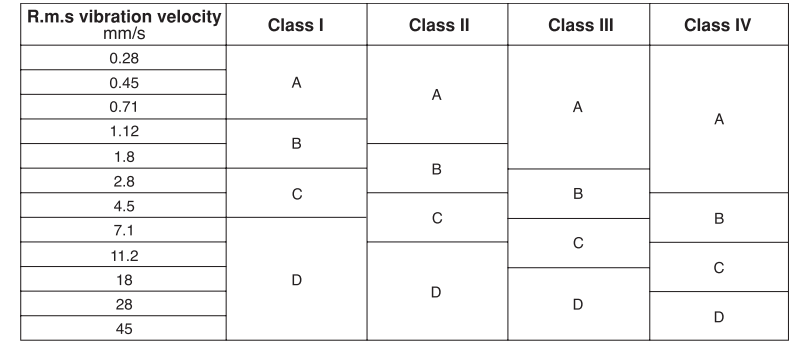
\includegraphics[scale=.5]{referencial/img/iso10816-1_randall_p146.png}
    \end{center}
    \fonte{\citeonline{Wu2013}.} 
    \label{fig:iso10816-1_randall_p146}
\end{figure}

Onde

\begin{itemize}
    \item A = bom estado
    \item B = aceitável
    \item C = apenas tolerável
    \item D = não permitido
    \item Classe I = pequenas máquinas (potência menor que $\SI{15}{\kilo\watt}$)
    \item Classe II = máquinas médias sem uma fundação especial (potência entre $\SI{15}{\kilo\watt}$ e $\SI{75}{\kilo\watt}$)
    \item Classe III = máquinas grandes sobre uma fundação rígida e pesada
    \item Classe IV = máquinas grandes sobre uma fundação flexível (turbomáquinas) 
\end{itemize}

Relembrando o que foi escrito anteriormente, é possível ver as assinaturas das falhas no espectro da vibração captada por um transdutor
que está acoplado no sistema. Quando uma falha de desalinhamento está presente, há um aumento de até duas vezes nas harmônicas de alta 
frequência, como pode ser visto na figura \ref{fig:misa_analog_p2} \cite{Sopcik2019}.

\begin{figure}[H]
    \caption{Indicação espectral de desalinhamento na velocidade.}
    \begin{center}
        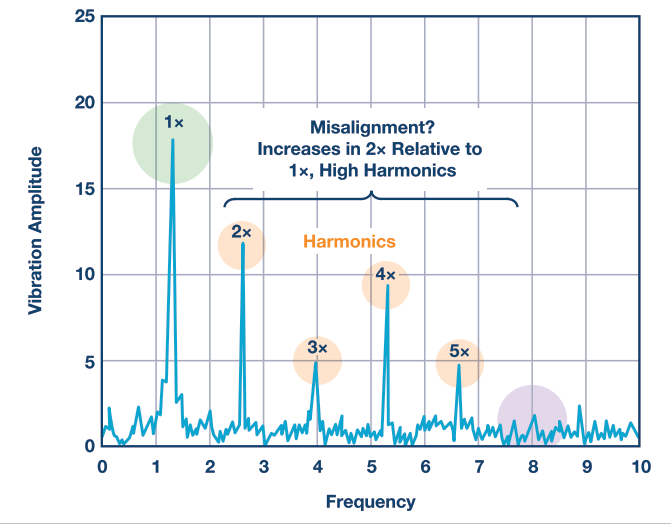
\includegraphics[scale=.4]{referencial/img/misa_analog_p2.png}
    \end{center}
    \fonte{\citeonline{Sopcik2019}.} 
    \label{fig:misa_analog_p2}
\end{figure}

Já quando uma falha de desbalanceamento está presente, há um aumento na harmônica principal da velocidade, em relação ao valor de base.
A figura \ref{fig:imbalance_analog_p2} exemplifica.

\begin{figure}[H]
    \caption{Indicação espectral de desbalanceamento na velocidade.}
    \begin{center}
        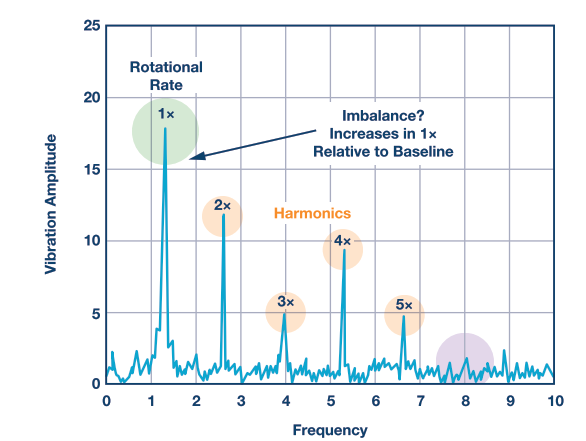
\includegraphics[scale=.5]{referencial/img/imbalance_analog_p2.png}
    \end{center}
    \fonte{\citeonline{Sopcik2019}.} 
    \label{fig:imbalance_analog_p2}
\end{figure}

No mesmo conceito, é possível identificar a assinatura de uma falha de rolamentos de acordo com o tipo de rolamento, velocidade de rotação
do motor, entre outras características. Uma tabela com estas frequências, se encontra na sequência na figura \ref{fig:bearing_table_analog_p3}


\begin{figure}[H]
    \caption{Tabela de frequências para falhas em rolamentos.}
    \begin{center}
        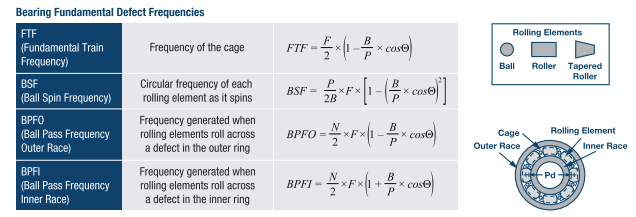
\includegraphics[scale=.7]{referencial/img/bearing_table_analog_p3.png}
    \end{center}
    \fonte{\citeonline{Sopcik2019}.} 
    \label{fig:bearing_table_analog_p3}
\end{figure}

Após a análise das falhas utilizando a vibração do sistema, é necessário fazer a mesma análise com a corrente elétrica na armadura, 
que será apresenta na subseção na sequência.


%----------------------------------------------------------------
% 
%----------------------------------------------------------------

\subsection{Análise de Corrente Elétrica }\label{sec:}

Como apresentado no circuito da figura \ref{fig:circuit_fitzgerald_p354}, variações na constituição mecânica de um motor elétrico de 
indução ocasionam variações na corrente e na tensão de entrada. Por exemplo o desbalanceamento, que pode ser uma anomalia no rotor,
tem uma assinatura específica no espectro da corrente de entrada \cite{Wu2013}.  A figura \ref{fig:fault_freq_randall_p55} contém as
frequências que estão associadas Às falhas em um rotor.

\begin{figure}[H]
    \caption{Ilustração com as frequências associadas às falhas em rotores ou estatores de motores elétricos.}
    \begin{center}
        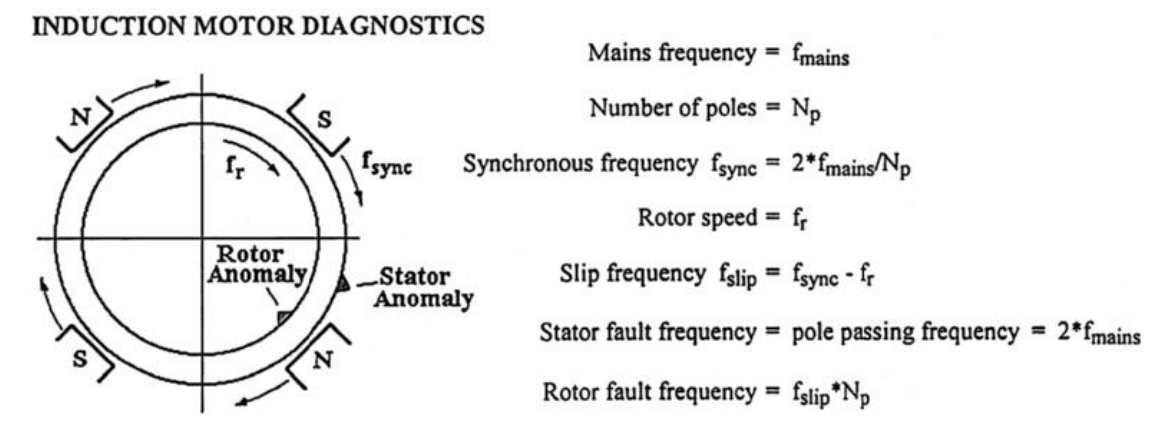
\includegraphics[scale=.35]{referencial/img/fault_freq_randall_p55.png}
    \end{center}
    \fonte{\citeonline{Wu2013}.} 
    \label{fig:fault_freq_randall_p55}
\end{figure}

Como é possível se estimar as frequências características de uma falha no rotor, é viável se criar um sistema que é capaz de detectar uma 
falha e indicá-la em tempo real se o espectro for analisado por algum algoritmo \cite{El1999}. A figura \ref{fig:current_benbouzid_p3} apresenta uma
técnica que utiliza esse conceito.

\begin{figure}[H]
    \caption{Proposta de sistema de diagnóstico utilizando a corrente do estator.}
    \begin{center}
        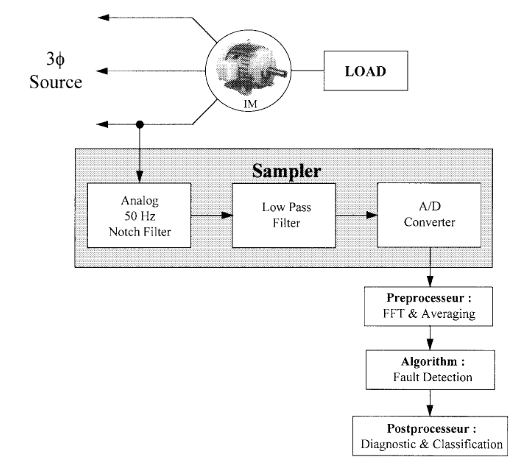
\includegraphics[scale=.5]{referencial/img/current_benbouzid_p3.png}
    \end{center}
    \fonte{\citeonline{El1999}.} 
    \label{fig:current_benbouzid_p3}
\end{figure}

Onde FFT é a transformada rápida de Fourier (\textit{Fast Fourier Transform}), que possibilita a obtenção do espectro com poucos recursos
computacionais e boa velocidade.

Após a apresentação das principais assinaturas que aparecem nos dados amostrados de motores elétricos de indução, técnicas de processamento
destes sinais são necessárias para a criação de um sistema autônomo e em tempo real. Estas técnicas estão descritas na próxima seção.


%++++++++++++++++++++++++++++++++++++++++++++++++++++++++++++++++
% 
%++++++++++++++++++++++++++++++++++++++++++++++++++++++++++++++++

\section{Técnicas Modernas de Processamento de Sinais}\label{sec:}

Com o objetivo de se detectar falhas e se obter um diagnóstico das mesmas, muitas técnicas já foram implementadas. Essas técnicas podem ser
não invasivas ou invasivas \cite{Gorbounov2018}. A figura \ref{fig:monitoring_methods_rilski_p78} apresenta algumas técnicas que são
utilizadas para detecção e diagnóstico de falhas.

\begin{figure}[H]
    \caption{Árvore de métodos de monitoramento de falhas em motores elétricos.}
    \begin{center}
        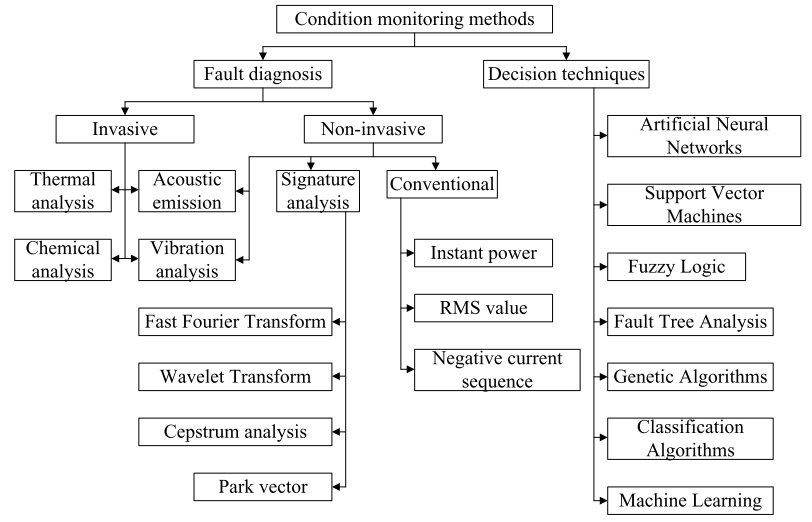
\includegraphics[scale=.5]{referencial/img/monitoring_methods_rilski_p78.png}
    \end{center}
    \fonte{\citeonline{Gorbounov2018}.} 
    \label{fig:monitoring_methods_rilski_p78}
\end{figure}

Dentre essas, a transformada rápida de Fourier (FFT) e CNN (\textit{Convolutional Neural network} - rede neural convolucional) 
serão descritas na sequência, adicionando mais uma técnica de análise de assinaturas que é a ICA (\textit{Indepent Compoent Analysys}
 - análise de componentes independentes). Além disso, o presente trabalho também aborda duas técnicas de aprendizagem de máquinas, que 
 é a t-SNE (\textit{t-Distributed Stochastic Neighbor Embedding} Incorporação Estocástica de Vizinhos com Distribuição T) e, por último, 
 a técnica K-means.


%----------------------------------------------------------------
% 
%----------------------------------------------------------------

\subsection{FFT}

FFT é um algoritmo muito eficiente que calcula a DFT (\textit{Discrete Fourier Transform} - Transformada discreta de Fourier), a qual 
pode ser descrita da seguinte forma \cite{Wu2013}:

\begin{equation}\label{eq:dft}
    G(k)=\frac{1}{N}\sum_{k=0}^{N-1} g(n)exp(-j2\pi kn/N)
\end{equation}

\begin{equation}\label{eq:dft}
    g(n)=\sum_{k=0}^{N-1} G(k)exp(j2\pi kn/N)
\end{equation}

Esta ferramenta é utilizada para se se representar no domínio da frequência, sinais discretos que estão no domínio do tempo. Isto 
possibilita analisar as assinaturas no espectro desses sinais, conforme descrito na seção anterior.


%----------------------------------------------------------------
% 
%----------------------------------------------------------------

\subsection{CNN}

CNNs são redes neurais artificiais (RNA) sem realimentação, inspiradas em redes neurais que compõe o córtex visual de mamíferos. Essa
técnica é largamente utilizada em processamento de imagens, principalmente em sistemas de reconhecimento em imagens e vídeos. Um exemplo
pode ser visto na figura \ref{fig:cnn_image_ince_p5}, onde um modelo que aceita uma imagem com 28 x 28 pixel. Cada camada subsequente é
subamostrada, dizimando a propagação 2D da camada anterior. O filtro 2D do kernel pe otimizado pelo algoritmo de retropropagação do erro, 
e os principais parâmetros de uma CNN são o tamanho do kernel e o fator de subamostragem \cite{Ince2016}.

\begin{figure}[H]
    \caption{Rede neural convolucional.}
    \begin{center}
        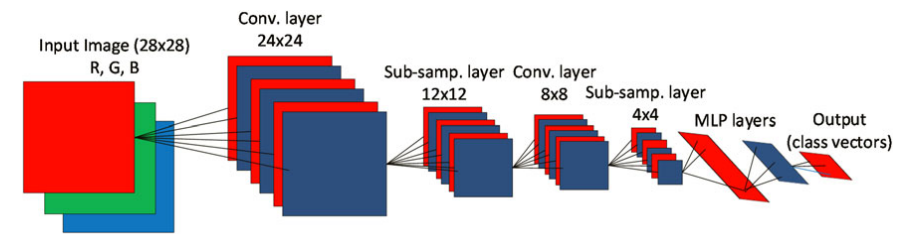
\includegraphics[scale=.4]{referencial/img/cnn_image_ince_p5.png}
    \end{center}
    \fonte{\citeonline{Ince2016}.} 
    \label{fig:cnn_image_ince_p5}
\end{figure}

Após a apresentação da técnica que permite reconhecer imagens, será apresentada a primeira técnica de aprendizagem de máquina, que se
encontra na próxima subseção.


%----------------------------------------------------------------
% 
%----------------------------------------------------------------

\subsection{ICA}

ICA foi criada para resolver o problema de separação de fontes desconhecidas, quando estes estão mixados. A técnica ICA utiliza o conceito
que as fontes estão estaticamente separadas. Se considerarmos o vetor de fontes de sinal $s=[s,...,s_i]^T$ e as observações
$X = [x_1,...,x_m]^T$ que geram uma matriz mixada A, seguindo a relação \cite{Duan2017}:

\begin{equation}\label{eq:ica_1}
    x = As
\end{equation}

A técnica ICA busca pela matriz W separadora, a qual pode recuperar as fontes estimadas, sendo representa da seguinte forma: 

\begin{equation}\label{eq:ica_2}
    s = A^{-1}X = WX
\end{equation}

A implementação escolhida para a ICA é a FastICA, a qual busca a maximização não Gaussiana da expressão $w^Tx$, onde w é o vetor linha
da matriz W, e $w_T$ é a sua transposta. Através do método Newton, podemos obter a matriz w da seguinte forma \cite{Duan2017}:

\begin{equation}\label{eq:ica_3}
    w_+ = w - \mu[E\{xg(w_Tx)-\beta w\}] /[E\{\hat{g}(w_Tx)-\beta\}]
\end{equation}

\begin{equation}\label{eq:ica_4}
    w^* = w^+/\parallel w^+\parallel
\end{equation}

Onde $w^*$ é o novo valor de w; $\mu$ é o passo da interação; $E\{.\}$ é o valor esperado; $g(.)$ é a derivada de $G(.)$; $G$ é uma
função constante e $\beta = E\{w^T Xg(w^T X)\}$.
Apresentadas as principais equações, o algoritmo pode ser visto na figura \ref{fig:fatica_fang_p3}.

\begin{figure}[H]
    \caption{Fluxograma do algoritmo FastICA.}
    \begin{center}
        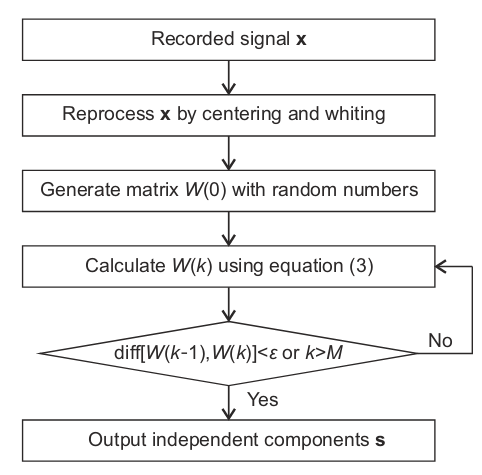
\includegraphics[scale=.5]{referencial/img/fatica_fang_p3.png}
    \end{center}
    \fonte{\citeonline{Duan2017}.} 
    \label{fig:fatica_fang_p3}
\end{figure}

A segunda técnica de aprendizagem de máquina encontra-se na subseção da sequência.


%----------------------------------------------------------------
% 
%----------------------------------------------------------------

\subsection{t-SNE}

É uma técnica não linear com o objetivo de reduzir a dimensionalidade de uma massa de dados. t-SNE é particularmente melhor que 
outras técnicas existentes para criar um único mapa que pode revelar estruturas de diferentes escalas. A técnica t-SNE começa com a 
conversão de dimensões superiores de distâncias Euclidianas entre dois dados em uma probabilidade condicional
$p_{j|i}$. A equação \ref{eq:t-sne_1} representa o cálculo, onde $\sigma$ é a variância \cite{VanDerMaaten2008}.

\begin{equation}\label{eq:t-sne_1}
    p_{j|i}=\frac{exp(-\parallel x_i-x_j\parallel^2/2\sigma_i^2)}{\sum_{k\ne i}{exp(-\parallel x_i-x_k\parallel^2/2\sigma_i^2)}}
\end{equation}

t-SNE utiliza a distribuição do tipo t com um grau de liberdade, com essa distribuição, a probabilidade $q_{ij}$ pode ser calculada como:

\begin{equation}\label{eq:t-sne_4}
    q_{ij}=\frac{(1+\parallel y_i-y_j\parallel^2)^{-1})}{\sum_{k\ne l}{(1 + \parallel y_k-y_l\parallel^2)^{-1}}}
\end{equation}

Com as duas equações, é possível calcular o gradiente de Kullback-Leibler  divergente entre P e a probabilidade Q, da seguinte forma:

\begin{equation}\label{eq:t-sne_5}
    \frac{\delta C}{\delta y_i} = 4 \sum_j{(p_{ij}-q_{ij})(y_i - y_j)(1+\parallel y_i-y_j\parallel^2)^{-1}}
\end{equation}

Após esclarecidas as equações, é possível apresentar o algoritmo que implementa a técnica, que está na figura \ref{fig:t-sne_algorithm_maaten_p9}.
\begin{figure}[H]
    \caption{Algoritmo simplificado da técnica t-SNE.}
    \begin{center}
        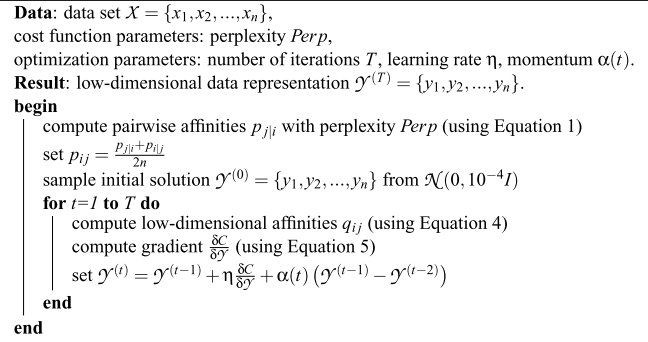
\includegraphics[scale=.45]{referencial/img/t-sne_algorithm_maaten_p9.png}
    \end{center}
    \fonte{\citeonline{VanDerMaaten2008}.} 
    \label{fig:t-sne_algorithm_maaten_p9}
\end{figure}

A presente técnica é a primeira sobre aprendizagem de máquina, onde a segunda está descrita na próxima subseção.


%----------------------------------------------------------------
% 
%----------------------------------------------------------------

\subsection{K-Means}

K-means é uma das técnicas mais populares de clusterização de dados, sendo publicada pela primeira vez em 1955. Sendo $X=\{x_i\}, i=1, ..., n$
n d-dimensões pontos para serem clusterizados em K clusters, onde $C = \{c_k, k=1, ..., K\}$. O algoritmo K-means encontra uma partição onde o erro quadrático entre a média 
empírica de um cluster e os pontos no cluster sejam minimizados. A média do cluster $c_k$ é $\mu_k$, definido da seguinte forma \cite{Jain2010}:

\begin{equation}\label{eq:k-means}
    J(c_k) = \sum_{x_j\in c_k} {\parallel x_i-\mu_k \parallel^2}
\end{equation}

E o objetivo é minimizar a seguinte expressão:

\begin{equation}\label{eq:k-means}
    J(c_k) = \sum_{k=1}^{K}\sum_{x_j\in c_k} {\parallel x_i-\mu_k \parallel^2}
\end{equation}

Com isso, os conceitos básicos das técnicas de processamento de sinais foram apresentados. A próxima seção contém algumas soluções
modernas para detecção e diagnóstico de falhas em motores elétricos.


%++++++++++++++++++++++++++++++++++++++++++++++++++++++++++++++++
% 
%++++++++++++++++++++++++++++++++++++++++++++++++++++++++++++++++

\section{Estado da Arte}

O estado da arte em detecção e diagnóstico de falhas em motores elétricos está no emprego de diversas técnicas numa mesma solução. Algumas 
utilizam técnicas clássicas com CNNs, outras empregam diversas técnicas modernas para se obter o resultado ótimo. A presente seção contem
algum exemplos que empregam novos arranjos de técnicas, as quais já foram discutidas anteriormente.

%----------------------------------------------------------------
% 
%----------------------------------------------------------------

\subsection{RNA}

O emprego de CNNs em classificação de imagens é muito utilizado para se classificar as assinaturas que foram geradas por alguma técnica
de processamento de sinais. A primeira solução que será apresentada, processa os sinais de corrente do motor via uma CNN de 1 dimensão,
conforme a figura \ref{fig:cnn_ince_p2}. Uma das principais características dessa técnica, é o emprego unicamente de uma CNN adaptativa,
não utilizando outras técnicas de processamento de sinais.


\begin{figure}[H]
    \caption{Diagrama de um sistema que utiliza CNN.}
    \begin{center}
        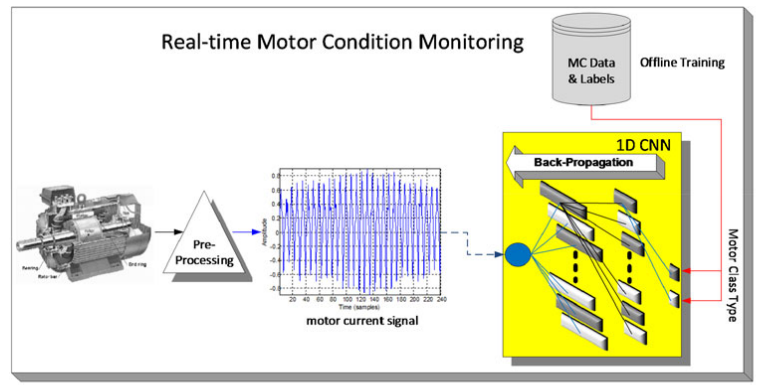
\includegraphics[scale=.45]{referencial/img/cnn_ince_p2.png}
    \end{center}
    \fonte{\citeonline{Ince2016}.} 
    \label{fig:cnn_ince_p2}
\end{figure}

Outra técnica que utiliza CNN é a que foi desenvolvida por \cite{Jeong2016}, onde uma imagem é gerada por um pré-processamento, que nada
mais é do que a criação de orbitais que são criados pela combinação de dois sensores que devem ter $\ang{90}$ entre eles. As expressões
que geram esses orbitais são as seguintes:

\begin{equation}\label{eq:}
    z(n) = x(n)+y(n)\dot j
\end{equation}

Onde x e y são os dados de vibração. E

\begin{equation}\label{eq:}
    Z(k) = \sum_{n=0}^{N-1}{z(n)e^{-j\frac{2\pi}{N}nk}}
\end{equation}

Uma aproximação para z(n), quando $\omega$ [e a velocidade angular, m é positivo e inteiro, $R_{m\omega_+}$ e $R_{m\omega_1}$ são números
complexos. 

\begin{equation}\label{eq:orbit}
    \hat{z}(n) = \sum_{m=1}^{N}(R_{m\omega_+}e^{jm\omega n}+R_{m\omega_-}e^{-jm\omega n})
\end{equation}

O offset pode ser removido via a subtração da média dos valores. Um exemplo de orbitais e suas falhas características pode ser visto
na figura \ref{fig:orbit_jeong_p3}.


\begin{figure}[H]
    \caption{Diagrama de uma técnica que utiliza classificação de orbitais com CNN.}
    \begin{center}
        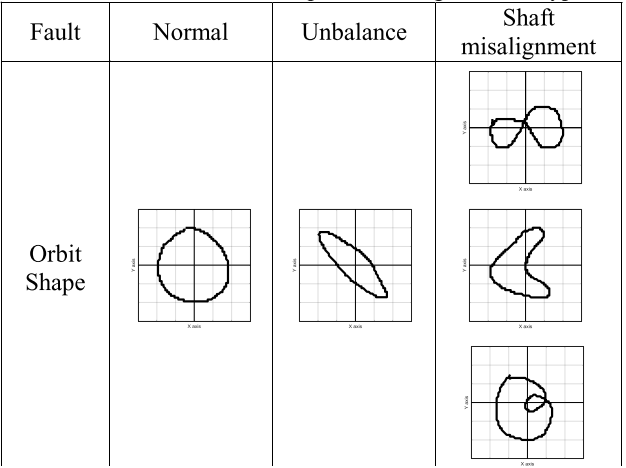
\includegraphics[scale=.45]{referencial/img/orbit_jeong_p3.png}
    \end{center}
    \fonte{\citeonline{Jeong2016}.} 
    \label{fig:orbit_jeong_p3}
\end{figure}

Após a obtenção desses orbitais e suas respectivas falhas, os autores treinaram uma CNN para reconhecer o orbital e classificar qual 
falha está se manifestando.

Outra técnica que emprega RNA, é a que está representada na figura \ref{fig:back-programation-zhang-p5}. Foram
testados vários tipos de RNAs com o objetivo de comparar o desempenho de cada uma delas, inclusive o proposto pelos autores \cite{Zhang2018}.

\begin{figure}[H]
    \caption{Técnica proposta por \citeonline{Zhang2018}.}
    \begin{center}
        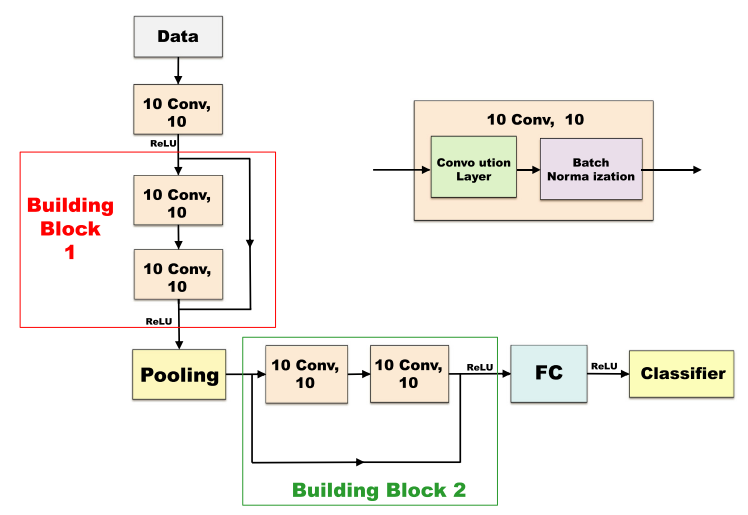
\includegraphics[scale=.35]{referencial/img/proposta_zhang_p4.png}
    \end{center}
    \fonte{\citeonline{Zhang2018}.} 
    \label{fig:proposta_zhang_p4.png}
\end{figure}

Ao testarem, obtiveram os seguintes resultados comparativos:

\begin{figure}[H]
    \caption{Resultados da técnica proposta por \citeonline{Zhang2018}.}
    \begin{center}
        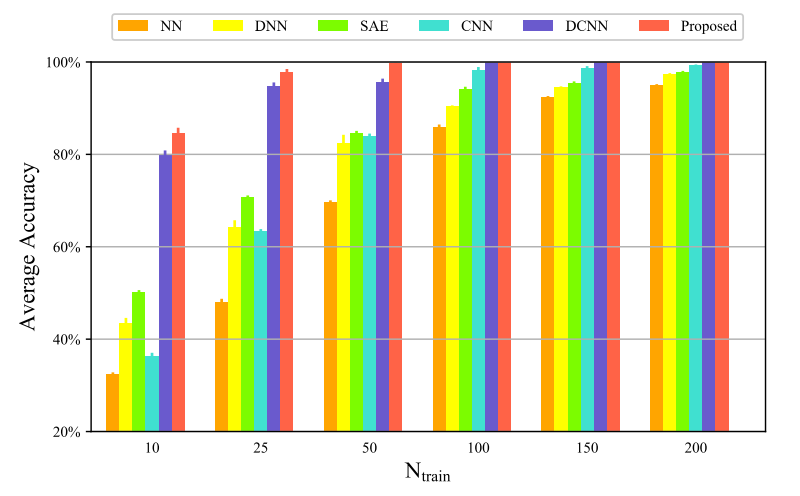
\includegraphics[scale=.35]{referencial/img/results_zhang_p7.png}
    \end{center}
    \fonte{\citeonline{Zhang2018}.} 
    \label{fig:back-programation-zhang-p5}
\end{figure}

Esses foram os principais casos de uso de RNA, com foco em CNN, onde é possível ver o melhor desempenho desse método sobre os demais
tipos de RNA. Na sequência, temos um método que combina FFT e ICA para detectar e classificar falhas.

%----------------------------------------------------------------
% 
%----------------------------------------------------------------

\subsection{ICA}

Essa técnica emprega 3 assuntos que já foram explicados anteriormente, incluindo FFT, ICA e RNA sobre o sinal de corrente
do motor. Os sinais que são aplicados no algoritmo FastICA, são o a saída da FFT normalizados e com um tamanho de 1024 amostras. 
A topologia se encontra na figura \ref{fig:ica_bracamonte_p4}. Por fim, ao se obter as características extra[idas pelo algoritmo FastICA,
a saída é aplicada em um RNA com o objetivo de classificar a saída.

\begin{figure}[H]
    \caption{Fluxograma de uma técnica que utiliza ICA.}
    \begin{center}
        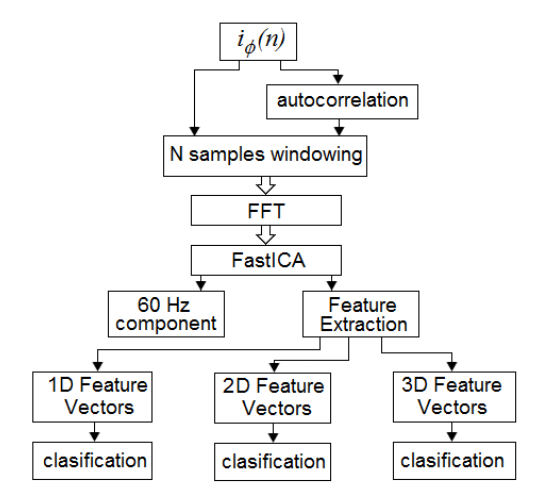
\includegraphics[scale=.5]{referencial/img/ica_bracamonte_p4.png}
    \end{center}
    \fonte{\citeonline{Garcia-Bracamonte2019}.} 
    \label{fig:ica_bracamonte_p4}
\end{figure}


Após elucidados os conceitos básicos sobre motores elétricos de indução, suas falhas, técnicas modernas de processamento de sinais e as 
técnicas que estão sendo empregadas na atualidade para se detectar e diagnosticar falhas, a proposta de solução do presente trabalho 
pode ser apresentada, que se encontra no próximo capítulo.